\section{Implementazione}
\subsection{\href{https://github.com/edoardosarri24/real-time-scheduling-simulator.git}{GitHub}}

\begin{frame}{Implementazione}
    \begin{columns}
        \begin{column}{.4\textwidth}
            \begin{block}{Scheduler}
                \begin{itemize}
                    \item Classe base che definisce la logica dello scheduling: \textit{Template Method}.
                    \item Classi concrete che implementano \texttt{assignPriority} e \texttt{addReadyTask}.
                \end{itemize}
            \end{block}
        \end{column}
        \begin{column}{.6\textwidth}
            \centering
            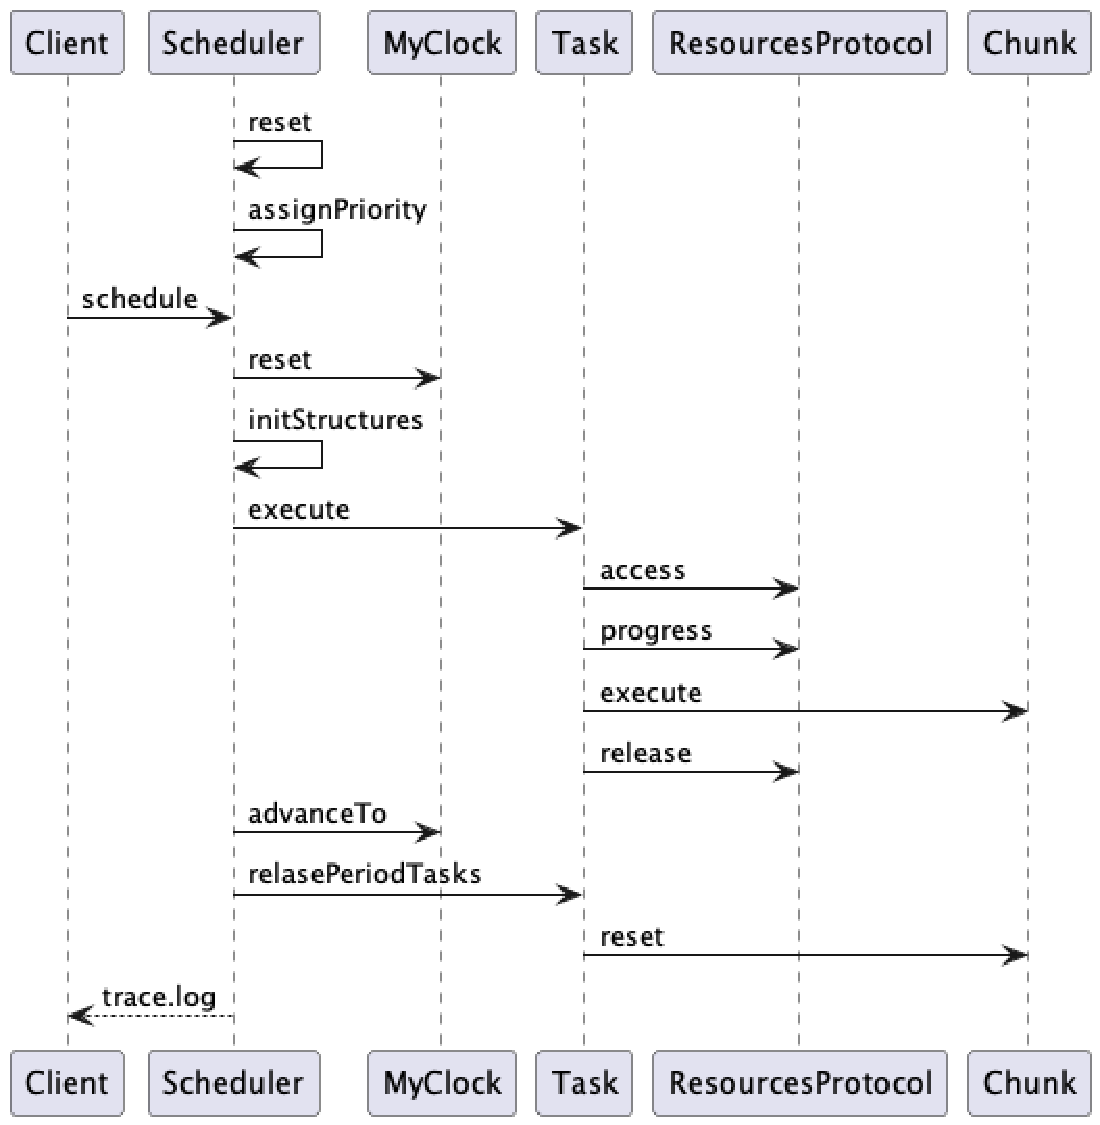
\includegraphics[width=\textwidth]{images/3-implementazione/sequence diagram.pdf}
        \end{column}
    \end{columns}
\end{frame}

\begin{frame}{Implementazione}
    \begin{block}{Resource Access Protocol}
        \begin{itemize}
            \item Necessario \texttt{NoResourceProtocol} quando non si hanno risorse condivise.
            \item Implementa i metodi di accesso, progresso e rilascio.
            \item PCP usa due strutture dati: \texttt{ceiling} e \texttt{busyResource}.
        \end{itemize}
    \end{block}
\end{frame}

\begin{frame}{Implementazione}
    \begin{block}{Clock}
        \begin{itemize}
            \item Gestione globale.
            \item Acceesso unificato tramite Singleton.
            \item Oggetti di tipo \texttt{Duration} di \texttt{java.time}.
        \end{itemize}
    \end{block}
    \begin{block}{Sampling}
        \begin{itemize}
            \item Libreria \texttt{Sirio}.
            \item Aggiunto \texttt{ConstantSampler} per il campionamento di di un tempo costante.
        \end{itemize}
    \end{block}
\end{frame}